\newpage
\hypertarget{M2TSettingUp vis}{}
\subsection{Setting up the Parser}
\visHeader

\begin{enumerate}

\item[$\blacktriangleright$] Your EA unexpanded project browser should now resemble Fig.~\ref{ea:mocaTagged}. You can see that your project is already populated
with the metamodel for our generic tree. To differentiate this from other trees (ANTLR parse tree and abstract syntax tree, XML DOM tree, \ldots) we refer to it
as \texttt{MocaTree}.

\begin{figure}[htpb]
\begin{center}
  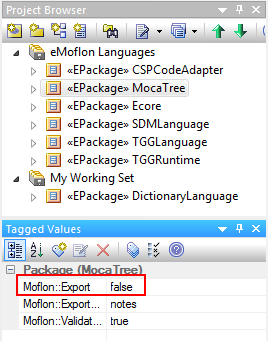
\includegraphics[width=0.4\textwidth]{ea_mocaTaggedValues}
  \caption{figureCaption}
  \label{ea:mocaTagged}
\end{center}
\end{figure}

\item[$\blacktriangleright$] Note that the \texttt{MocaTree} package has a special tagged value \texttt{Moflon::Export} set to \texttt{false}\footnote{The
``Tagged Values'' window can be opened by going to ``View/Tagged Values''}. This ensures that the package is \emph{ignored} when exporting. As with all standard
metamodels (e.g., Ecore or the SDM metamodel) the \texttt{MocaTree} package in EA should be regarded as read-only and is only required in the EA project so that
SDMs can refer to the classes defined in the package. The corresponding Java code is provided by our Eclipse plugin and is added automatically to the Java build
path whenever necessary.

\item[$\blacktriangleright$] Go ahead and inspect the \texttt{MocaTree} metamodel (Fig.~\ref{ea:mocaTree}). It basically combines concepts from a filesystem
(folders and files), XML concepts (text-only nodes and attributes), and a general indexed\footnote{The index attribute in \texttt{TreeElement} can be used to
demand a certain \emph{order} of nodes in an SDM, which is otherwise not guaranteed by default (order is in general non-deterministic).} containment hierarchy.

\begin{figure}[htpb]
\begin{center}
  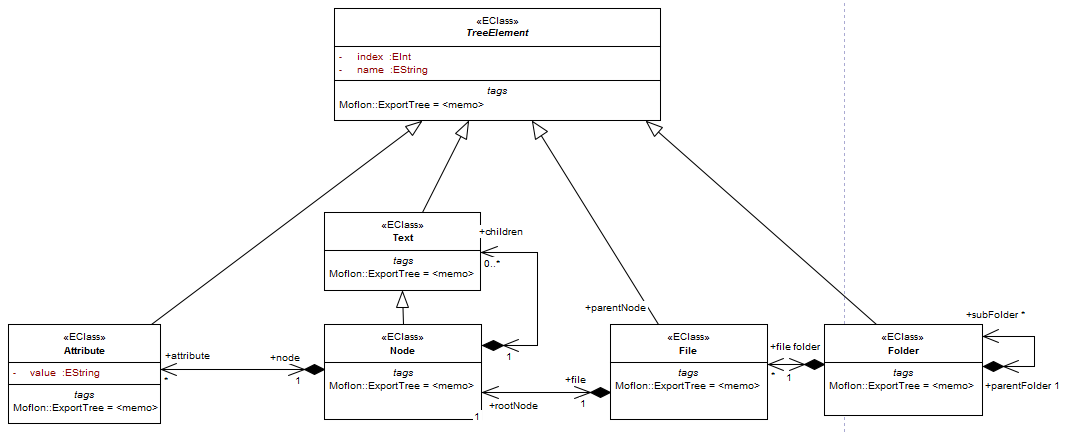
\includegraphics[width=\textwidth]{ea_metamodelMocaTree}
  \caption{figureCaption}
  \label{ea:mocaTree}
\end{center}
\end{figure}
 
\newpage

\item[$\blacktriangleright$] Add a package to your \texttt{My Working Set} node named \texttt{Dic\-tion\-ary\-Code\-Adapter}. Add a new \texttt{TGG Schema}
diagram to it with the same name (Fig.~\ref{ea:tggDiagram}), and set its \texttt{Source Project} as \texttt{Dictionary Language}, and the \texttt{Target
Project} as \texttt{MocaTree}. Your project browser should then closely resemble Fig.~\ref{ea:adapterPackageBrowser}. ({\bf WRONG TGG?})

\begin{figure}[htpb]
\begin{center}
  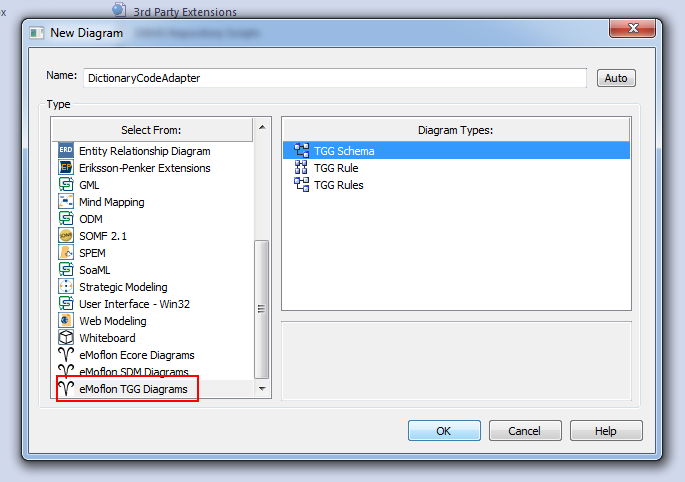
\includegraphics[width=0.9\textwidth]{ea_tggDiagram}
  \caption{figureCaption}
  \label{ea:tggDiagram}
\end{center}
\end{figure}

\begin{figure}[htpb]
\begin{center}
  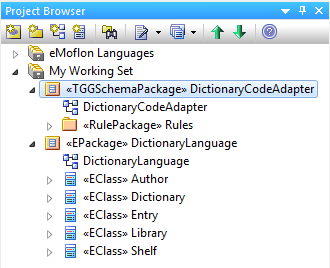
\includegraphics[width=0.45\textwidth]{ea_packageCodeAdapter}
  \caption{figureCaption}
  \label{ea:adapterPackageBrowser}
\end{center}
\end{figure}

Our conventions and workflow state that this \emph{code adapter} is a package that contains the tree-to-model transformation logic. This could be integrated
directly in the corresponding metamodel (\texttt{Dic\-tion\-ary\-Language}), but here a separation makes sense as there could be \emph{different} code adapters
for the \emph{same} language.

\item[$\blacktriangleright$] Validate your entire project as usual\footnote{Refer to Part II, Section 2.8 for details} and ensure that your refreshed Eclipse
workspace closely resembles Fig.~({\bf not sure yet.. we DO need some sort of diagram though}). Note especially the library nodes (\texttt{Moflon} and
\texttt{Moca}) that reference jars for all required dependencies. 

\item[$\blacktriangleright$] Right-click on \texttt{DictionaryCodeAdapter} one more time and choose ``Add Parser/Unparser'', this time from the eMoflon context
menu (Fig~ %\ref{fig:moca-1-AddParserAndUnparserWizard}).
 
\item[$\blacktriangleright$] In the wizard dialogue (Fig %\ref{fig:moca-2-AddParser}),
enter ``dictionary'' as file extension, and check the boxes \texttt{Create Parser} and \texttt{Create Unparser} with \texttt{ANTLR} chosen as corresponding
 technology in both cases.  Click \texttt{Finish}.

\end{enumerate}

If everything has been installed and set up properly, parser and unparser stubs should be generated and \texttt{ANTLR} should automatically build the
corresponding Java code as depicted in Fig.~%\ref{fig:moca-3-WizardResult}.

